\section{Implementace}

\subsection{Volba technologií a struktura projektu}
Aplikaci jsem rozdělil na backend a frontend. Backend bude zajišťovat veškerou \uv{vědeckou} práci, tedy extrakci melodie, správu databáze skladeb a samotné vyhledávání podobnosti. Backend tyto služby poskytne frontendu pomocí REST API. Na frontendu bude poté implementováno uživatelské rozhraní pro vyhledávání.

Pro backend se přirozeně nabízel jazyk Python, který disponuje mnoha knihovnami pro vědeckou práci, zároveň se dalo jednoduše experimentovat pomocí Jupyter notebooku, než všechno implementovat na ostro. Nejdříve jsem se však snažil najít Python knihovnu pro práci s MIDI soubory, abych extrakci nemusel implementovat ve frontendu (zde se nabízela Javascriptová knihovna \textit{Tone.js}, která je schopna MIDI soubory konvertovat na JSON). Pro Python jsem našel knihovnu \textit{Mido}, která k MIDI souborům přistupuje více low-level způsobem. I přes tento fakt jsem si vybral Python s tím, že knihovnu \textit{Mido} vyzkouším. Jako web framework jsem zvolil \textit{Django}, který se postará o samotné API a jakoukoliv práci s databází.

Pro frontend jsem zvolil Javascriptový framework \textit{Vue 3} s grafickou knihovnou \textit{Vuetify}.

\subsection{Extrakce melodie}
Nejdříve bylo potřeba extrahovat melodii z MIDI souborů. MIDI soubory se mohou skládat z několika stop (tracks). Každá stopa se pak skládá z tzv. zpráv (messages). Existují různé druhy zpráv s různými parametry (standard je dobře popsaný např. na stránce \cite{midi-standard})
S knihovnou \textit{Mido} \cite{mido} můžeme MIDI soubor jednoduše načíst a vypsat všechny zprávy z nějaké stopy: 

\begin{figure}[!ht]
    \begin{minted}[bgcolor=LightGray]{python}
from mido import MidiFile

# Load midi file
midi = MidiFile("../midi/piano_midi_de/bach/bach_846.mid")

# Print all messages in the second track
for message in midi.tracks[1]:
    print(message)
    \end{minted}
\end{figure}

\begin{figure}[!ht]
    \begin{minted}[bgcolor=LightGray]{python}
MetaMessage('midi_port', port=0, time=0)
MetaMessage('track_name', name='Piano right', time=0)
program_change channel=0 program=0 time=0
control_change channel=0 control=7 value=100 time=0
control_change channel=0 control=10 value=64 time=0
control_change channel=0 control=91 value=127 time=0
MetaMessage('text', text='bdca426d104a26ac9dcb070447587523', time=0)
note_on channel=0 note=67 velocity=56 time=241
note_on channel=0 note=67 velocity=0 time=120
note_on channel=0 note=72 velocity=60 time=0
note_on channel=0 note=72 velocity=0 time=120
note_on channel=0 note=76 velocity=63 time=0
note_on channel=0 note=76 velocity=0 time=108
...
note_on channel=0 note=72 velocity=0 time=0
MetaMessage('end_of_track', time=0)
    \end{minted}
\end{figure}
\pagebreak
Na výstupu kódu lze vidět, že některé zprávy nastavují parametry skladby (\lstinline{MetaMessage}, \lstinline{program_change}, \lstinline{control_change}) a některé zprávy určují noty, které se mají přehrávat (\lstinline{note_on}).

Každá zpráva má dále atribut \lstinline{time}, který určuje odchylku této zprávy od předchozí v tickích. Pokud má zpráva hodnotu \lstinline{time} nastavenou na 0, zpráva se spustí ve stejnou dobu, jako ta předchozí. Seznam zpráv je tedy vypsán sekvenčně s tím, že každá zpráva nenese absolutní časovou hodnotu, ale pouze odchylku od té předchozí zprávy.

Ve zprávě \lstinline{note_on} se výška noty určuje atributem \lstinline{note}. Na stránkách standardu MIDI \cite{midi-standard} lze nalézt tabulku pro zjištění, kterou notu dané číslo reprezentuje. Atribut \lstinline{velocity} určuje hlasitost dané noty.

Ve výpisu si můžete všimnout, že nota se na nějakou dobu zapne nastavením \lstinline{velocity} na nějakou kladnou hodnotu, a posléze se nota vypne opět zprávou \lstinline{note_on} s \lstinline{velocity} nastavenou na 0. Tento fakt je matoucí, jelikož existuje i zpráva \lstinline{note_off}, kterou se noty také dají vypínat. Existují tedy dva různé způsoby vypínání not, na což je potřeba brát ohled při zpracovávání MIDI souborů z různých zdrojů. Častěji se na vypínání not používá \lstinline{note_on}, avšak jsem zjistil, že např. program pro tvorbu hudby \textit{FL Studio} používá \lstinline{note_off}.

Dalším problémem, se kterým jsem se při extrakci potýkal, byl ten, že každá zpráva (i \lstinline{MetaMessages}, které nemají mít s melodií nic společného) mohou mít nastavenou časovou odchylku \lstinline{time} na větší než 0. Při extrakci více stop najednou pak nastaly problémy, jelikož jsem hodnotu \lstinline{time} kontroloval pouze u zpráv \lstinline{note_on}.

Práce s touto knihovnou tedy byla zapeklitější, avšak mi umožnila lépe poznat formát MIDI zevnitř a dala mi větší kontrolu při extrakci melodie. Na samotnou extrakci jsem použil metodu výšek.


\subsection{Vyhledávání podobných melodií}
V backendu jsem implementoval automatickou extrakci melodií ze všech skladeb ze stránky piano-midi.de do databáze. LCS a DTW jsem implementoval dynamickým programováním. Při vyhledávání se dotaz porovná se všemi skladbami v databázi, přičemž se každá skladba rozdělí na segmenty stejné délky, jakou má dotaz.

Segmentaci skladeb jsem nejdříve zkoušel implementovat metodou \uv{sliding window} -- segmenty mají opět stejné délky, jako dotaz, akorát např. druhý segment nezačíná na konci prvního segmentu, nýbrž druhou notou celé skladby. Tímto způsobem lze najít potencionálně lepší výsledky, avšak je výpočetně složitejší, než jednoduše rozdělit skladbu na na sebe navazující segmenty -- při jednoduchém postupu je složitost porovnání dotazu ($m$) se všemi segmenty skladby ($n_1, n_2, \ldots$) $O(mn_1 + mn_2 + \ldots) = O(m(n_1 + n_2 + \ldots)) = O(mn)$, kdežto metoda sliding window má složitost $O(m^2(n - m))$. Kvůli větší složitosti jsem od této metody musel upustit, jelikož vyhledávání trvalo příliš dlouho.

Každá skladba se tedy rozdělí na na sebe navazující segmenty stejné délky, jako dotaz. V každé skladbě algoritmus vyhledá segment s nejlepší hodnotou LCS/DTW. Algoritmus pak vrátí seznam skladeb seřazený podle nejpodobnějšího segmentu.

\subsection{Uživatelské rozhraní}
Pro frontend jsem si vybral Javascriptový framework Vue, který si zakládá na rozložení UI do menších celků (tzv. komponent) a reaktivitě -- prvky na stránce automaticky reagují na změnu vnitřních dat. Díky těmto vlastnostem jsem mohl jednoduše sestavit tzv. sekvencer pro zadávání vstupní melodie pro vyhledávání. Sekvencer sestává z ovládacích prvků (pro přehrání či vyčištění zadané melodie) a z mřížky pro zadávání melodie. Díky Vue dokážu reprezentovat zadanou melodii polem, na jehož změnu celý sekvencer reaguje. To také zjednodušuje implementaci několika operací -- např. vyčištění zadané melodie = nastavení všech prvků pole na počáteční hodnotu.

Díky sekvenceru si uživatel svůj dotaz může přehrát a dále ladit už před tím, než jej vyhledá. Další výhoda spočívá v tom, pokud uživatel chce nahrát jako dotaz MIDI soubor. Místo toho, aby se po nahrání souboru hned spustilo vyhledávání, se z něj nejdříve vyextrahuje melodie, která se následně zobrazí v sekvenceru. Uživatel tak může zkontrolovat, jestli se MIDI soubor zpracovává správně a případně může melodii opět ladit bez potřeby nějakého externího programu.

\begin{figure}[!ht]
    \centering
    \caption{Sekvencer se zadanou melodií, která se právě přehrává}
    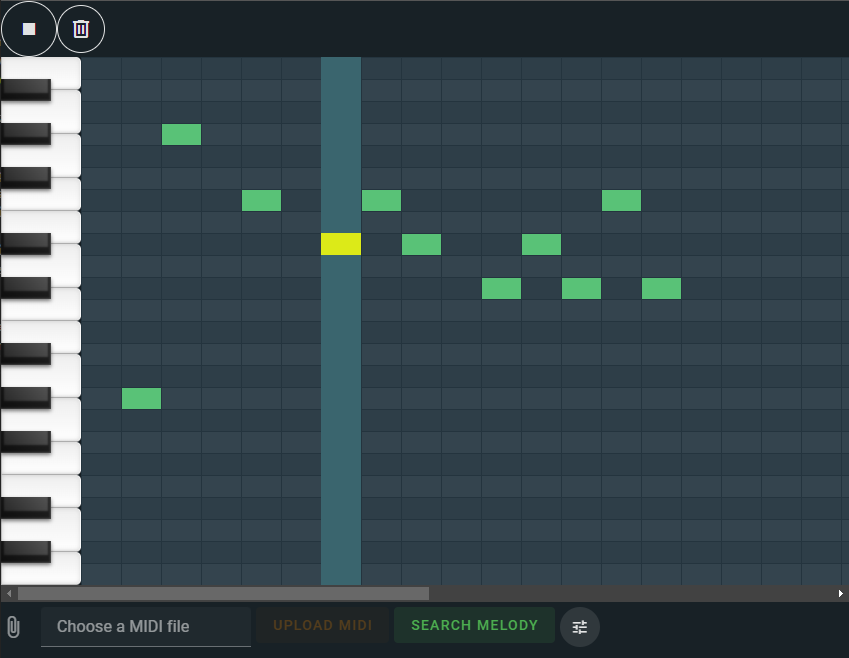
\includegraphics[width=\textwidth]{images/seq_playing.png}
\end{figure}

V pravé části rozhraní se nachází panel s nastaveními vyhledávání -- zvolení funkce LCS/DTW a počet vrácených nejlepších výsledků. V dolní části rozhraní se po dokončení vyhledávání zobrazí seřazené výsledky.

\begin{figure}
    \centering
    \caption{Všechny prvky rozhraní}
    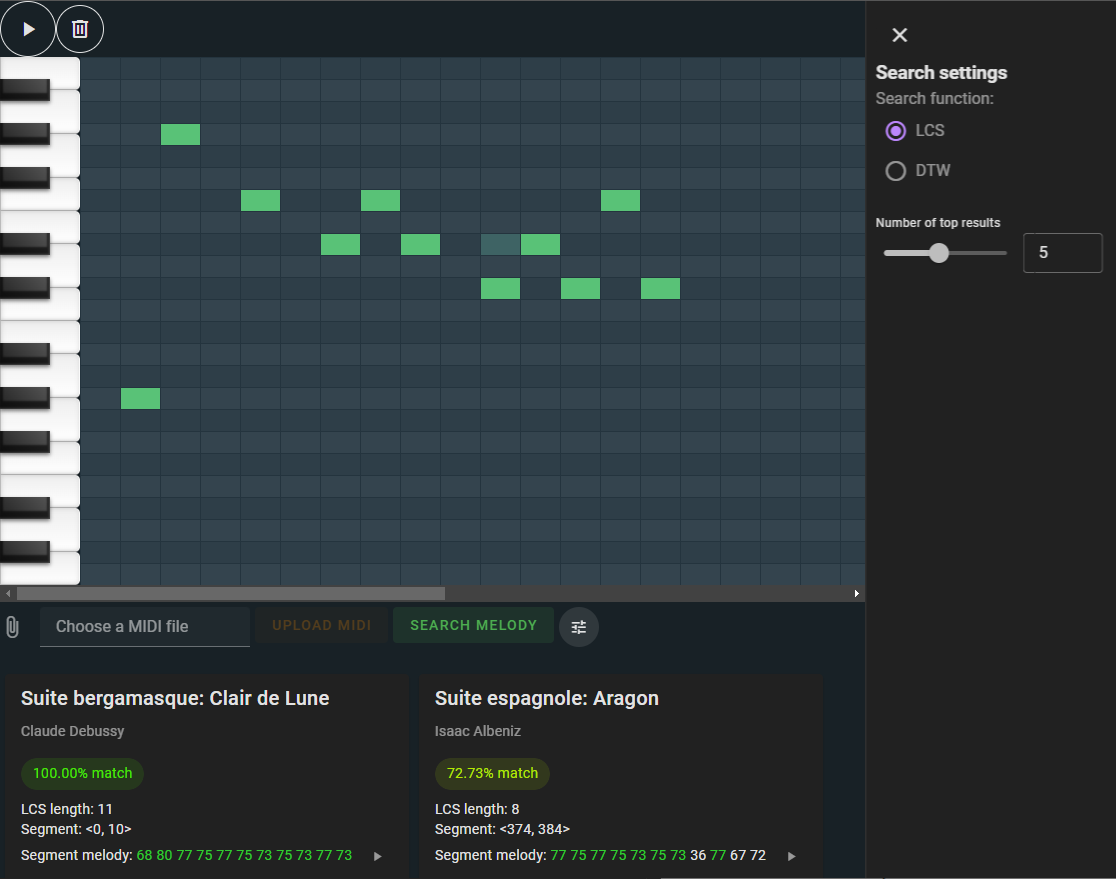
\includegraphics[width=\textwidth]{images/interface.png}
\end{figure}
\pagebreak